% !TeX spellcheck = hu_HU
% !TeX encoding = UTF-8


\chapter{Nagyvállalati környezetek ismertetése}

A vállalatok egyre nagyobb hangsúlyt fektetnek az informatikai rendszereik fejlesztésére és karbantartására, üzemeltetésére. Az ezek által nyújtott szolgáltatások sok esetben jelentős könnyebbséget jelentenek egyes üzleti folyamatokban, és a megfelelően automatizált munkafolyamatok csökkentik az egyes munkavállalók által elvégzendő manuális feladatokat, és adott esetben az ügyfelek számára is segítséget nyújthatnak. Fontos tisztában lenni azonban azzal, hogy ezek a megoldások csak akkor működnek jól a mindennapi használat során, ha sikerül biztosítani a megfelelő rendelkezésre állást, tehát egy -- a vállalat munkavállalói által a munkához nélkülözhetetlen -- szolgáltatásnak munkaidőben folyamatosan elérhetőnek kell lennie. Előfordulhatnak olyan igények is, amik miatt bizonyos, a vállalat működésének szempontjából nélkülözhetetlen szolgáltatásoknak folyamatosan elérhetőnek kell lenniük, mert a működésük nem munkaidőhöz kötött (ilyen lehet például a szervezet weboldala, illetve levelezőszervere).  Emellett a fent említett informatikai rendszerek karbantartásának is sokszor észrevehetetlennek kell lennie, azaz egy esetleges frissítés nem hátráltathatja a munkavégzést és a rendelkezésre állást. Az ilyen helyzetek kezelésére számos megoldás jött létre, ezek közül néhányat ismertetni fogok a következő fejezetben.

Egy másik fontos szempont a nagyvállalati rendszerek üzemeltetése -- és általában informatikai megoldások üzemeltetése és használata során -- ami napjainkban egyre nagyobb figyelmet kap, az IT-biztonság kérdése. A rendszerüzemeltetőknek tisztában kell lenniük a potenciális veszélyekkel, veszélyforrásokkal és fel kell készülniük egy esetleges támadásra, annak kezelésére. Sokszor hallhatunk a rendszeres biztonsági mentések fontosságáról, és ezek típusairól, követelményeiről. Egy jól bevett gyakorlat például az úgynevezett \textit{\mbox{3-2-1}}~mentési stratégia, ami egy jó kiindulási alapul szolgálhat minden szervezet számára a biztonsági mentésekhez~\cite{Backblaze321}.
A megoldás elnevezése az alábbi elvekből származik:
\begin{itemize}
	\item három példány az adatokról,
	\item két különböző eszközön (akár más típusú adathordozókon, pl. SSD, HDD, mágnesszalag -- ez segít az adathordozóra jellemző esetleges hibák hatásának csökkentésében),
	\item egy példányt földrajzilag különböző helyen tároljunk (pl. a cég székhelyén legyenek az eredeti adatok és még egy mentés, további egy példányt pedig tároljunk adatközpontban, vagy vegyünk igénybe harmadik féltől biztonságimentés-szolgáltatást)~\cite{Seagate321}.
\end{itemize}

A biztonsági mentések elvégzésére és automatizálására többféle megoldást választhat a szervezet az igényeihez igazodva. Bevett szokás például, hogy a cégen belüli mentéseket valamilyen mentést támogató vagy akár teljesen automatizáló szoftverrel oldják meg (például Bareos, Bacula, BackupPC). Az ilyen megoldások üzembe helyezése nehezebb lehet, mintha például csak egyéni scriptekkel hajtanánk végre a mentéseket, de hosszabb távon mégis célszerű lehet megfelelően konfigurálni őket, mert könnyebben kezelhetővé teszik egy komplex infrastruktúrában található gépek adatainak mentését, illetve az egyszer megírt konfigurációs fájlok több gépen is felhasználhatóak. Mindezek mellett ezek a szoftverek általában rendelkeznek valamilyen grafikus felhasználói felülettel (pl. webes interfész), amely tovább egyszerűsíti a mentések készítését, valamint szükség esetén a mentés visszaállítását.

% TODO: Bareos web UI kép lecserélése
\begin{figure}[!ht]
	\centering
	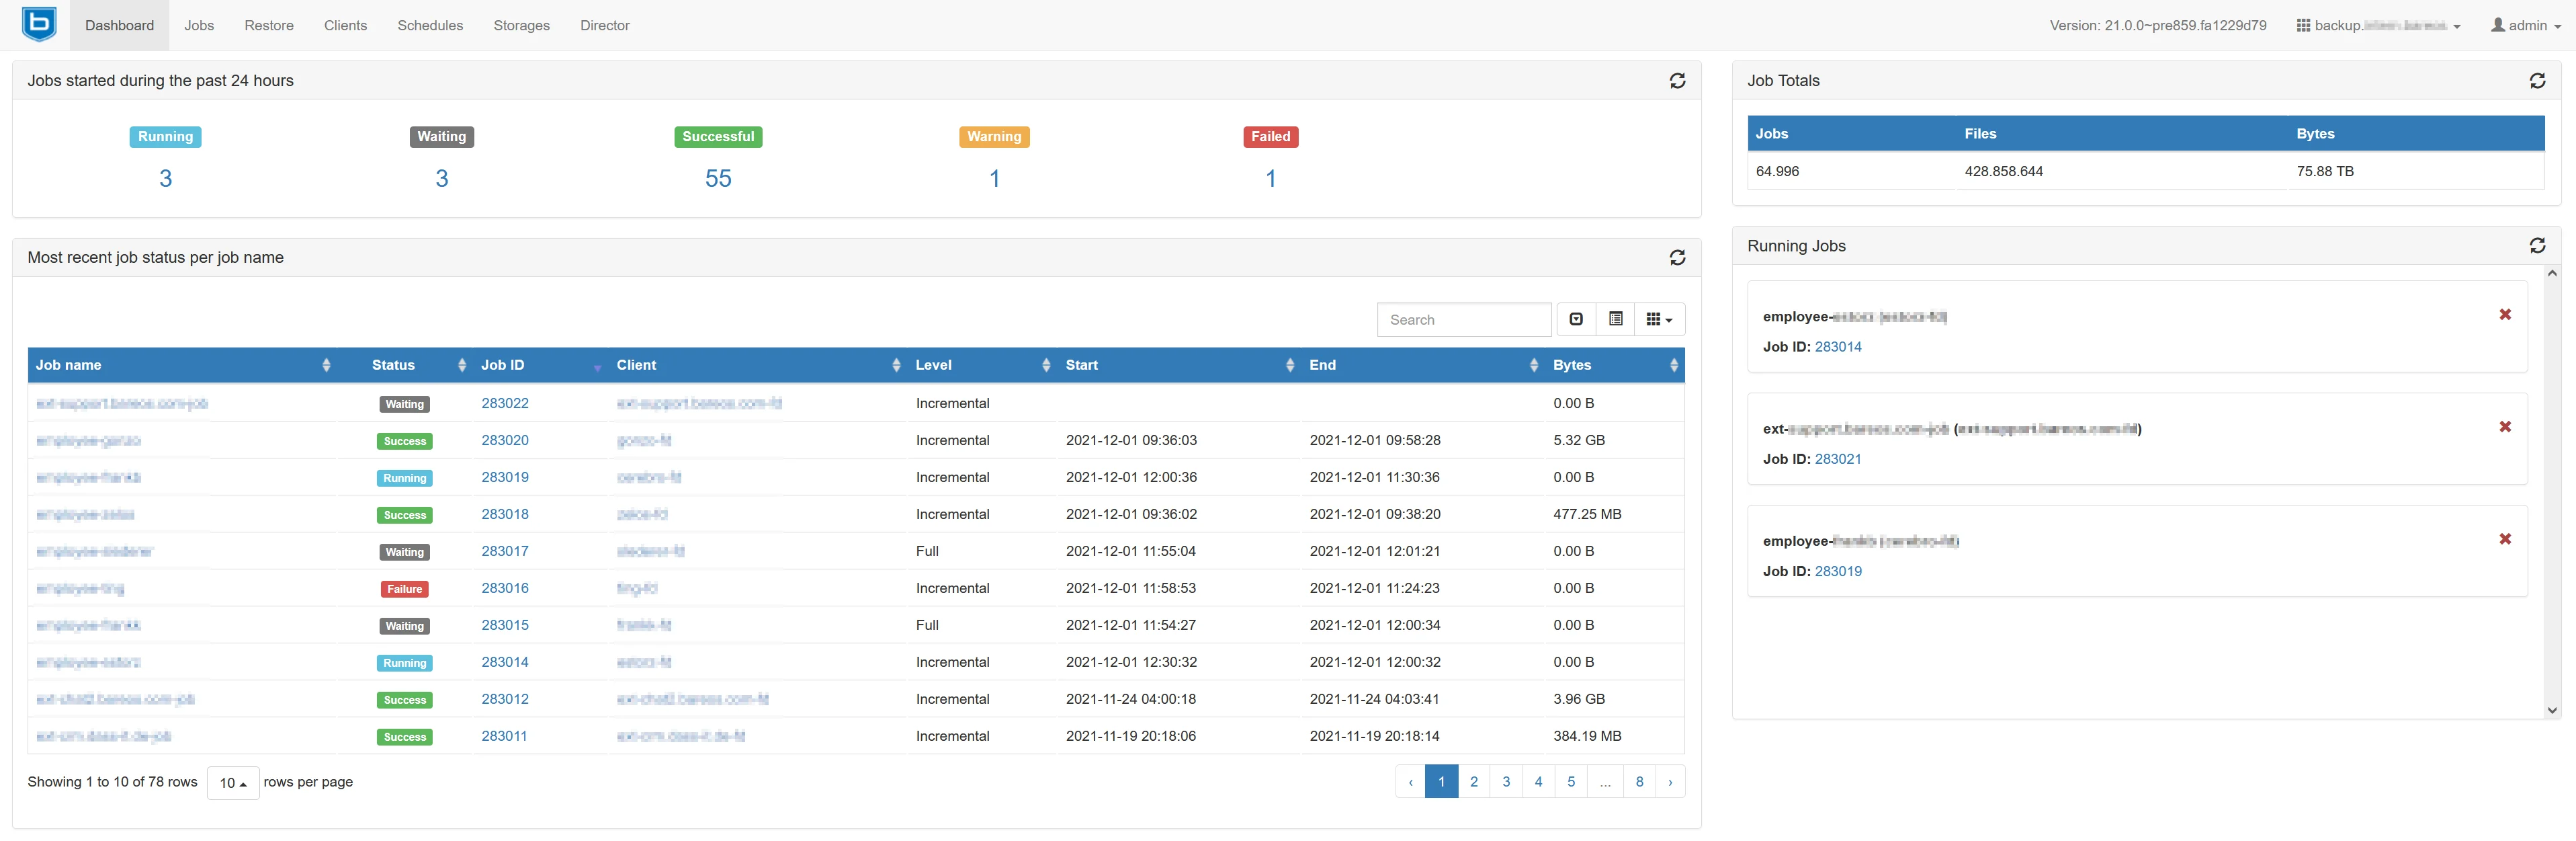
\includegraphics[width=150mm, keepaspectratio]{figures/bareos-dashboard.png}
	\caption{A Bareos biztonsági mentéseket végző program webes felületének részlete. Forrás: \url{https://www.bareos.com/bareos-webui-modules/}}
	\label{fig:bareos}
\end{figure}

A legtöbb hétköznapi felhasználó számára ismeretlen vagy meglepő lehet, hogy maga az internet és az ezen keresztül elérhető szolgáltatások -- gondoljunk például az Ügyfélkapura vagy az internetbank-szolgáltatásokra -- nagyon komplex rendszerek nem csak szoftveres, hanem informatikai infrastruktúra szempontjából is. A legtöbb ilyen szolgáltatás egy adatközpontban lévő szerveren fut, ami a beérkező kérésekre ad válaszokat. Ezt a folyamatot úgy is felfoghatjuk, hogy az ilyen szolgáltatások felhasználói lényegében az adott szolgáltató (a fenti példánál maradva a Magyar Állam és az adott bankok) számítógépeivel kommunikálnak.

Ezek a szervergépek több lényeges különbséggel is bírnak a személyi számítógépekkel szemben. Egyik legfontosabb tulajdonságuk, hogy hibatűrőek bizonyos hardverhibákat illetően: szinte minden főbb komponensből legalább kettő áll rendelkezésre, így ha az egyik meg is hibásodik, akkor a hiba elhárításáig a beépített redundancia miatt a gép képes tovább funkcionálni, általában a felhasználók felé észrevétlenül, míg a gép üzemeltetői figyelmeztetést kapnak a hiba típusáról és a kapcsolódó tennivalókról.
% TODO: kép redundáns dolgokról (pl. hálózati kártya, PSU), és hibajelző elemekről (pl. CPU fault, RAM-hiba, diszk hiba)

